\documentclass{beamer} 
\usecolortheme{lily}
\usepackage{graphicx}

\title{Scala, a Scalable Language} 
\author{Alan Dipert} 
\date{September 10th, 2009} 

\begin{document} 
\maketitle 

\begin{frame} 
\frametitle{What Scala Is}
\begin{columns}[c]
  \column{0.5in}
    
\includegraphics[width=1.0in]{graphics/scala_logo.png} 
  \column{2.5in}
    \begin{itemize}
      \item<1-> Multi-paradigm: integrates features of object oriented and functional programming
      \item<2-> Statically typed
      \item<3-> Seamless Java interoperability
      \item<4-> Open source (BSD License)
      \item<5-> Latest of several JVM languages from creator Martin Odersky and team at EPFL
      \item<6-> Cool: \tt{def fact(x:BigInt):BigInt = if (x==0) 1 else x * fact(x-1)}
    \end{itemize}
\end{columns}
\end{frame} 

\begin{frame} 
\frametitle{Object Oriented Programming in Scala}
\begin{columns}[c]
  \column{1.0in}
    \includegraphics[width=1.8in]{graphics/oop_dot.pdf} 
  \column{2.0in}
    \begin{itemize}
      \item<1-> Classes are "blueprints" for objects, objects are "instances of" classes
      \item<2-> Classes and objects similar to Java...
      \item<3-> ...except "everything is an object."  No simple types like Java
      \item<4-> Automatic getters/setters (like :attr\_accessor in Ruby)
      \item<5-> Uses "Singleton objects" instead of allowing classes to have static members.
      \item<6-> "Traits," behaviors added to classes and objects, simplify traditional multiple inheritance problems
    \end{itemize}
\end{columns}
\end{frame} 

\begin{frame}[fragile]
\frametitle{Class Definition in Scala}
{\tt \tiny
\begin{semiverbatim}
\uncover<1->{//Person objects take the name 'n' and the age 'a' in the constructor}
\uncover<1->{class Person(n:String, a:Int) \{}
\uncover<2->{  //name and age are immutable instance values}
\uncover<2->{  val name = n}
\uncover<2->{  val age = a}
\uncover<3->{  //Person provides its own toString method that returns something sensible}
\uncover<3->{  override def toString = "My name is %s and I'm %d years old.".format(name,age)}
\uncover<1->{\}}
\uncover<4->{}
\uncover<4->{val thePrez = new Person("Barrack Obama", 48)}
\uncover<5->{}
\uncover<5->{println(thePrez toString)}
\uncover<5->{//prints "My name is Barrack Obama and I'm 48 years old."}
\end{semiverbatim}
}
\end{frame} 

\begin{frame}[fragile]
\frametitle{Inheritance in Scala}
{\tt \tiny
\begin{semiverbatim}
\uncover<1->{class Person(n:String, a:Int) \{}
\uncover<1->{  val name = n}
\uncover<1->{  val age = a}
\uncover<1->{  override def toString = "My name is %s and I'm %d years old.".format(name,age)}
\uncover<1->{\}}
\uncover<2->{}
\uncover<2->{class Student(u:String, n:String, a:Int) extends Person(n,a) \{}
\uncover<3->{  val school = u}
\uncover<3->{  override def toString = super.toString+" I go to %s.".format(school)}
\uncover<3->{\}}
\uncover<4->{}
\uncover<4->{val alan = new Student("RIT", "Alan Dipert", 25)}
\uncover<5->{}
\uncover<5->{println(alan toString)}
\uncover<5->{//prints "My name is Alan Dipert and I'm 25 years old. I go to RIT."}
\end{semiverbatim}
}
\end{frame} 

\begin{frame}[fragile]
\frametitle{Traits in Scala}
{\tt \tiny
\begin{semiverbatim}
\uncover<1->{class Person(n:String, a:Int) \{}
\uncover<1->{  val name = n}
\uncover<1->{  val age = a}
\uncover<1->{  override def toString = "My name is %s and I'm %d years old.".format(name,age)}
\uncover<1->{\}}
\uncover<1->{}
\uncover<1->{class Student(u:String, n:String, a:Int) extends Person(n,a) \{}
\uncover<1->{  val school = u}
\uncover<1->{  override def toString = super.toString+" I go to %s.".format(school)}
\uncover<1->{\}}
\uncover<2->{}
\uncover<2->{trait Cool \{}
\uncover<2->{  override def toString = super.toString+" And I'm cool."}
\uncover<2->{\}}
\uncover<2->{}
\uncover<3->{trait LaidBack \{}
\uncover<3->{  override def toString = super.toString+" And I'm laid back."}
\uncover<3->{\}}
\uncover<4->{}
\uncover<4->{val ferris = new Student("Shermer High", "Ferris Bueller", 17) with LaidBack with Cool}
\uncover<5->{}
\uncover<5->{println(ferris toString)}
\uncover<5->{//"My name is Ferris Bueller and I'm 17 years old. I go to Shermer High. And I'm laid back. And I'm cool."}
\end{semiverbatim}
}
\end{frame} 

\begin{frame} 
\frametitle{Object Oriented Programming Conclusions}
\begin{columns}[c]
  \column{1.0in}
    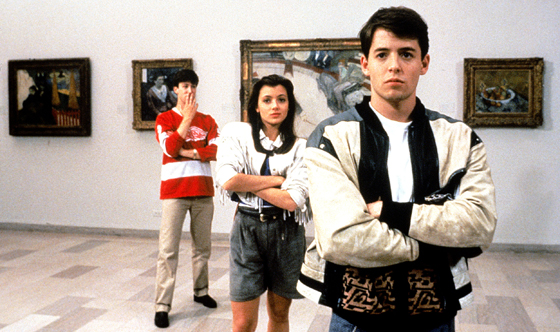
\includegraphics[width=1.5in]{graphics/ferris.jpg} 
  \column{2.0in}
    \begin{itemize}
      \item<1-> Scala's object system gives you a lot of control
      \item<2-> It feels much more like Ruby or Python than Java or C++
      \item<3-> It's a carefully designed fusion of useful features and Java compatibility
      \item<4-> Like a lot of Scala, you can start by doing things the Java way
    \end{itemize}
\end{columns}
\end{frame} 

\begin{frame} 
\frametitle{Functional Programming in Scala}
\begin{columns}[c]
  \column{1.0in}
    
\includegraphics[width=1.5in]{graphics/hat.png} 
  \column{2.0in}
    %\begin{itemize}
      %\item<1-> Scala's object system gives you a lot of control
      %\item<2-> It feels much more like Ruby or Python than Java or C++
      %\item<3-> It's a carefully designed fusion of useful features and Java compatibility
      %\item<4-> Like a lot of Scala, you can start by doing things the Java way
    %\end{itemize}
\end{columns}
\end{frame} 

\end{document} 
